\Header{Начало работы в Free Pascal}

\header{Установка}
Free Pascal (сокращённо FP) — это свободное кросс-платформенное программное обеспечение, поэтому его можно легко
скачать с официального сайта, можно свободно распространять, и можно установить на все современные операционные
системы.

Чтобы установить FP под Windows, скачайте программу установки с официального сайта
\verb`http://freepascal.org` (что не очень тривиально), или из другого надежного источника (участники моего курса на informatics могут скачать установщик со странички курса).
Установите FP с помощью этой  программы, ничего сложного в установщике нет. Я точно не помню, создаёт ли установщик ярлык на 
рабочем столе; если нет, то найдите исполняемый файл FP. Путь к нему имеет вид 
\verb`C:\FPC\bin\i386-win32\fp.exe` (начальная часть может отличаться в зависимости от того, куда 
установлен FP, у меня он установлен в \verb`C:\FPC`). Удобнее всего вынести ярлык к FP на рабочий 
стол или ещё куда-нибудь, чтобы было легко запускать.

Если вы работаете в другой операционной системе, то разберитесь, как установить FP, самостоятельно. В Linux,
например, FP есть в репозиториях всех ведущих дистрибутивов.

\header{Первая программа}
Запустите Free Pascal. Появится окошко, похожее на показанное на рис. \ref{fpc-0}а или \ref{fpc-0}б. Если появилось окошко, показанное
на рис. \ref{fpc-0}а, то в FP, в меню File выберите пункт New — окошко примет вид, показанный на рис. \ref{fpc-0}б.
В этом окне наберите следующий текст (рис. \ref{first-prg}):
\begin{verbatim}
begin
writeln('This is test! ',2*2);
end.
\end{verbatim}
(Здесь \verb`'` "--- это символ, называемый апостроф. Он находится в латинской раскладке клавиатуры на той же клавише, что и русская буква э. В разных шрифтах он выглядит по-разному, но обычно как половина символа кавычек.)

Убедитесь, что опечаток нет. Сохраните программу: нажмите F2 или выберите пункт меню File --- Save. FP предложит
выбрать имя файла для сохранения, для первой программы можно выбрать любое имя.


\begin{figure}[p]
\centerline{
а)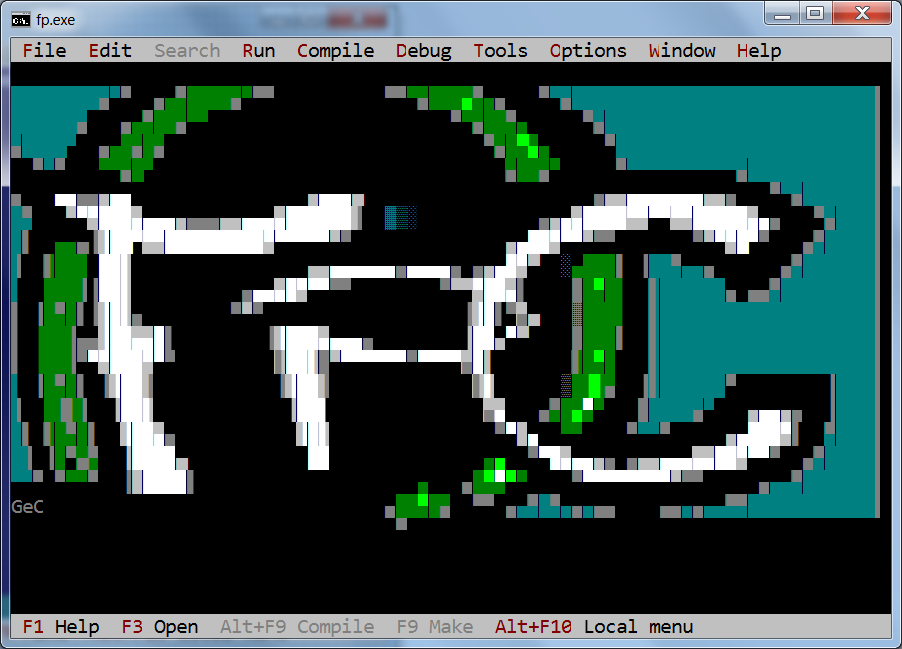
\includegraphics[width=8cm]{fpc-0.png}
а)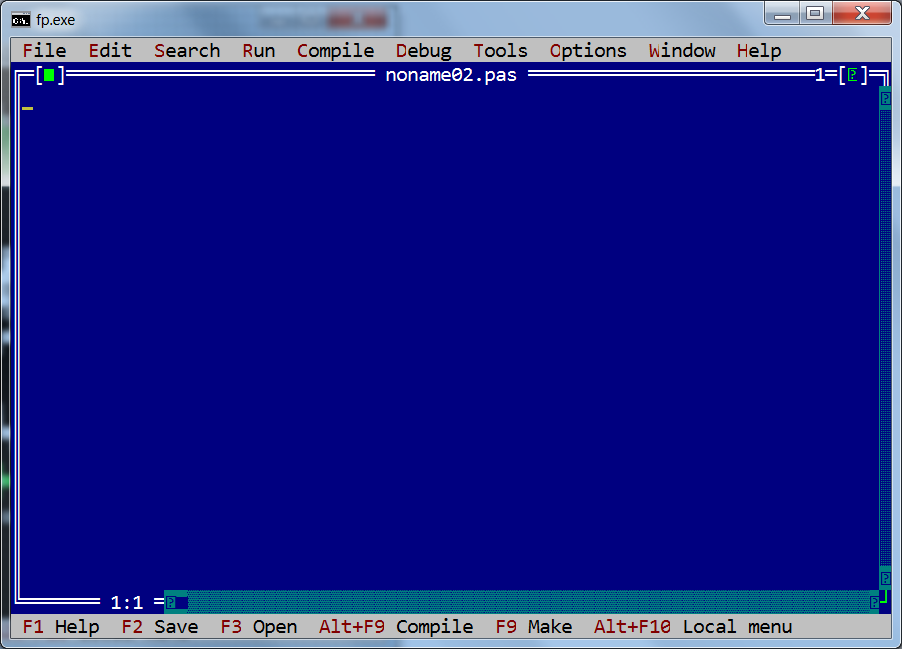
\includegraphics[width=8cm]{fpc-noname.png}
}
\caption{Основное окно FP}
\label{fpc-0}
\end{figure}

\begin{figure}
\centerline{
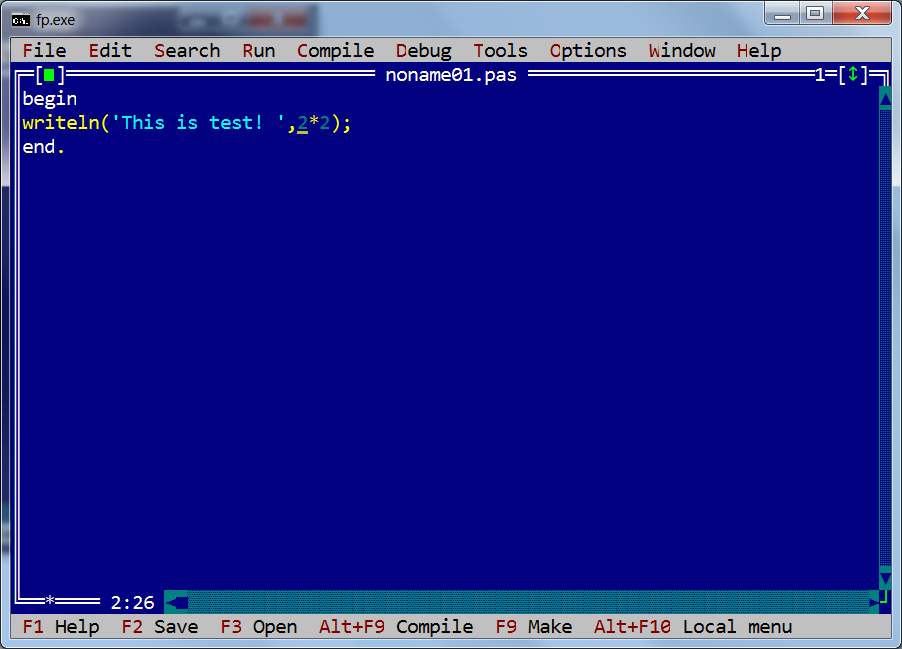
\includegraphics[width=8cm]{first-prg.png}
}
\caption{Простейшая программа}
\label{first-prg}
\end{figure}

После этого запустите программу, нажав Ctrl-F9 или в меню Run выбрав пункт Run. (Если вы не сохранили программу заранее, то FP предложит вам сохранить её перед запуском. Сохраните.) Окно FP на мгновение
пропадёт, может быть, вы успеете увидеть за ним другое, чёрное, окошко, после чего окошко FP с набранной программой (рис. \ref{first-prg}) появится обратно. Это значит, что программа успешно выполнилась. Если вместо этого вы видите
картинку, похожую на рис. \ref{ce}а, это значит, что в программе есть ошибки. Про это ниже (раздел \ref{sec:ce}), а пока будем считать,
что ошибок нет и программа успешно выполнилась.

\begin{figure}
\centerline{
а)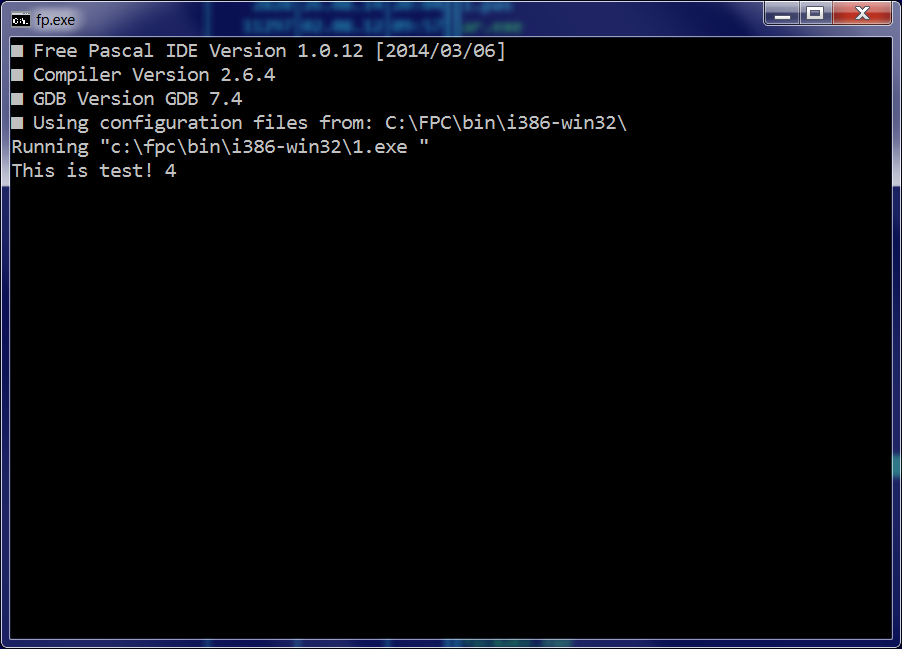
\includegraphics[width=8cm]{output-1.png}
б)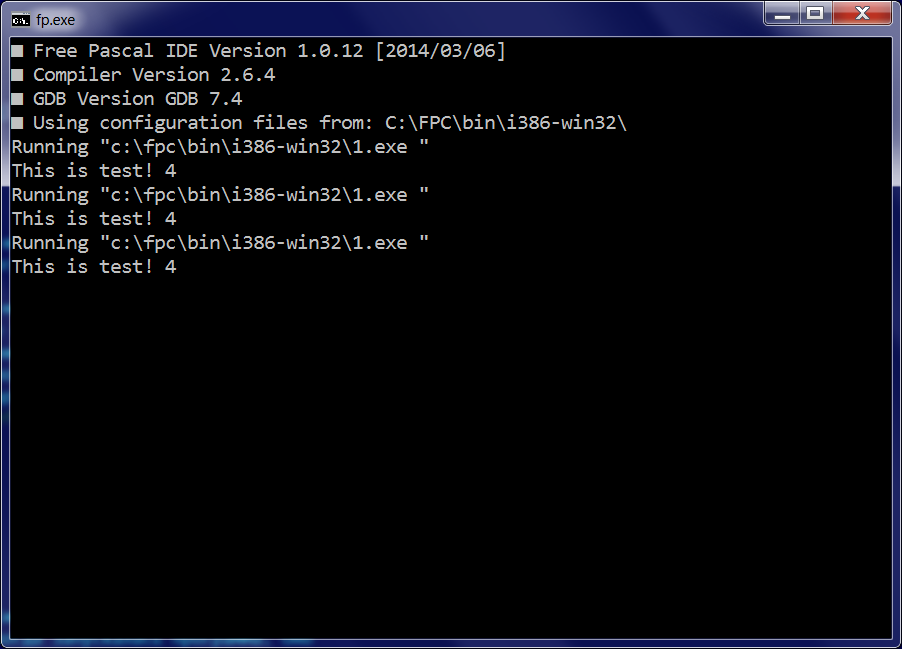
\includegraphics[width=8cm]{output-3.png}
}
\caption{Вывод программы}
\label{output}
\end{figure}

Нажмите Alt-F5 или в меню Debug выберите пункт User screen. Синее окошко редактора пропадёт, а появится
то самое чёрное окошко, которое вы могли заметить, когда запускалась программа. Оно показано на рис. \ref{output}а. В нем,
во-первых, виден заголовок FP — строчки, начинающиеся с квадратика. Их FP выводит один раз при каждом запуске
редактора. Далее идёт строка ``\verb`Running "c:\fpc\bin\i386-win32\1.exe "`'' (путь может быть другой, в зависимости от того, куда сохранена ваша программа). Это строка была выведена в тот момент, когда FP начал запускать
вашу программу. И, наконец, есть строка ``\verb`This is test! 4`'', которую и напечатала наша программа. Почему она
напечатала именно это, обсудим чуть ниже.

На чёрном экране нажмите любую клавишу — вы вернётесь обратно в редактор. Позапускайте программу (Ctrl-F9)
ещё несколько раз и посмотрите на результаты (Alt-F5). Вы увидите картину, показанную на рис.~\ref{output}б: FP каждый раз
печатает строку ``\verb`Running...`'' перед запуском программы, потом программа печатает свою строку.
Вывод программы перемешивается с выводом FP — ничего страшного, это нормально.

\begin{figure}
\centerline{
а)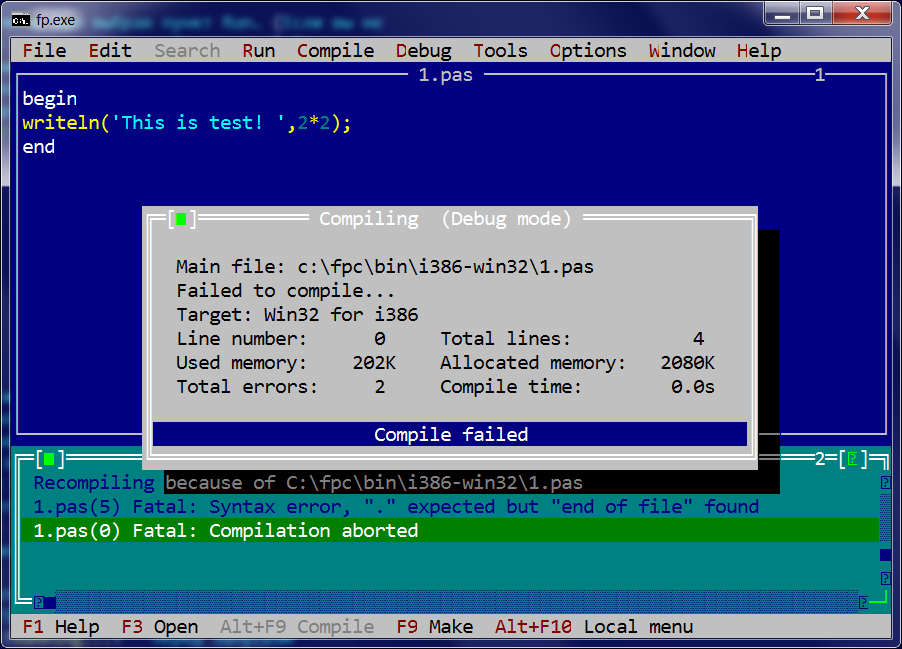
\includegraphics[width=8cm]{fp-ce.png}
б)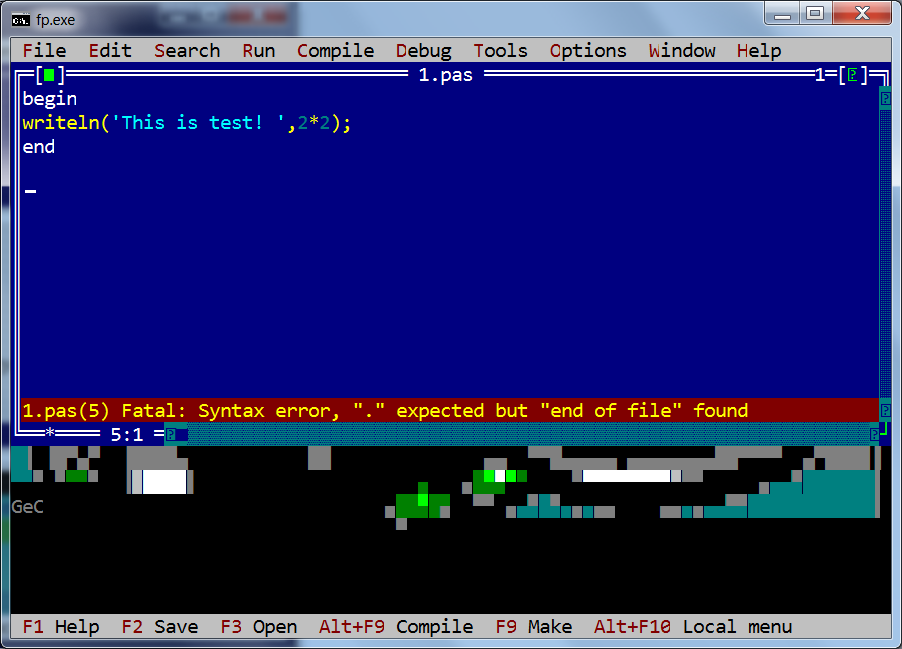
\includegraphics[width=8cm]{fp-ce-expl.png}
}
\caption{Ошибка компиляции}
\label{ce}
\end{figure}

\header{Ошибки компиляции}
\label{sec:ce}
Компиляцией называется (это не совсем точное определение) процесс перевода программы из текстового вида (``исходного кода'') в такой вид, в котором её можно запустить на компьютере (``исполняемый файл''). Когда вы нажимаете
Ctrl-F9, происходит сначала компиляция, а потом полученный исполняемый файл запускается. Соответственно, система, которая выполняет компиляцию, называется компилятором; это — основная часть Free Pascal.

В вашей программе могут быть серьёзные ошибки — такие, что компилятор даже не может скомпилировать программу, и уж тем более её невозможно запустить (а могут быть и не столь серьёзные — программа запустится, но
выдаст неверный результат). В таком случае компилятор выдаст сообщение, похожее на показанное на рис. \ref{ce}а.
В этом случае следует поступать следующим образом. Не вчитывайтесь в то, что показано в этом окошке. Вместо
этого нажмите два раза Enter — FP поставит вас курсор на то место, где он обнаружил ошибку, и напишет красную
строчку с сообщением об ошибке, см. рис \ref{ce}б.

Пока для вас важным будет то, куда компилятор поставил курсор "--- примерно в том месте и ошибка. Важен также
текст (``сообщение об ошибке''), выданный на красной строчке (``\verb`Syntax error, ...`''). Поначалу сообщения об ошибке
сложно понимать, но со временем вы выучите наиболее часто встречающиеся и будете сразу понимать, что не так.
В данном случае, если вы знаете английский, то сообщение об ошибке понятно: «Синтаксическая ошибка, ``.'' ожидалась, но ``конец файла'' найден». Очевидно, мы забыли точку после end. Если вы не так хорошо знаете английский,
то вам придётся внимательно всматриваться в программу и искать ошибку, хотя это, конечно, не очень сложно. На
самом деле, если даже вы неплохо знаете английский, вы все равно далеко не все сообщения об ошибках сможете понимать "---
поначалу смысл многих сообщений будет загадочен, и вам придётся все равно просто внимательно искать опечатки
и ошибки. Со временем, независимо от того, хорошо ли вы знаете английский, список наиболее частых ошибок вы
выучите.

Обратите ещё внимание, что компилятор поставил курсор не туда, где мы забыли точку, а дальше. Дело в том, что, строго говоря, между \verb`end` и точкой можно было ещё поставить сколько угодно пробелов и переводов строк. Так оказалось (точнее, это я специально сделал), что после \verb`end` в этом примере у меня шли ещё несколько пробелов и переводов строк. Их компилятор честно пропустил, ожидая найти точку, но файл кончился, а точки так и не нашлось. Поэтому компилятор сообщил об ошибке, но уже на конце файла, а не сразу после \verb`end`. 

Вывод из этой ситуации такой: компилятор не телепат и не может точно определить, где вы допустили ошибку. Он устанавливает курсор туда, где текст программы впервые разошёлся с правилами языка. Поэтому бывает, что на самом деле ваша ошибка чуть выше, чем курсор (а иногда "--- и намного выше). Но тем не менее место, куда компилятор ставит курсор, обычно бывает полезно при поиске ошибки.

Попробуйте в своей программе поделать разные ошибки и посмотрите, как на них отреагирует FP. 
(Особенно внимательные смогут заметить, что эту программу можно слегка изменить определённым образом так, 
что будет казаться, что появилась ошибка, но компилятор не будет ругаться. Если вы найдёте, как это 
сделать, то знайте, что это правда, это действительно не ошибка, но так писать просто не принято.)

\header{Как работает эта программа}

Давайте разберём, как эта программа работает. Напомню её текст:
\begin{verbatim}
begin
writeln('This is test! ',2*2);
end.
\end{verbatim}


Вообще, любая программа "--- это, в первую очередь, последовательность команд, которые программист 
даёт компьютеру, а компьютер будет последовательно их выполнять. В языке программирования паскаль 
начало этой последовательности команд (т.е. начало программы) обозначается словом \verb`begin`, а 
конец "--- словом \verb`end.` (с~точкой на конце!). Это "--- обязательные элементы любой программы, поэтому они есть и в 
нашей программе. 

Между ними в нашей программе одна команда "--- \verb`writeln('This is test! ',2*2);`. Команда 
\verb`writeln` обозначает ``вывести на экран'' (английское слово `write' обозначает писать, а ln 
"--- это сокращение от line "--- строка). В скобках после слова \verb`writeln` указываются, как 
говорят, \textit{аргументы} команды. Они разделяются запятыми, в данном случае у команды два 
аргумента: первый "--- \verb`'This is test! '`, и второй "--- \verb`2*2`. После команды ставится 
точка с запятой; вообще, это общее правила паскаля "--- после каждой команды должна идти точка с 
запятой (есть некоторые исключения, но пока они нам не важны).

Если аргументом команды является некоторая строка, заключённая в апострофы (символы \verb`'`), то 
команда \verb`writeln` выводит эту строку на экран как есть (без апострофов). Поэтому первым делом наша команда 
выводит на экран текст ``\verb`This is test! `'' (включая пробел на конце!).

Вторым аргументом команды \verb`writeln` в нашем примере является арифметическое выражение 
\verb`2*2`. Если аргументом команды (любой команды, не обязательно именно \verb`writeln`, 
просто других мы 
пока не знаем) является арифметические выражение, то компьютер сначала вычислит его, а потом 
передаст команде. Поэтому в данном случае сначала компьютер вычислит $2\cdot 2$, получит 4, а потом 
передаст результат команде \verb`writeln`, которая выведет его на экран. 

В итоге получается, что наша программа выводит \verb`This is test! 4`.

\header{Использование паскаля как калькулятора}

Таким образом можно использовать паскаль как калькулятор. Например, если надо посчитать значение 
выражения $7+3\cdot(8-2)$, то можно написать команду \verb`writeln(7+3*(8-2));`, не забыть 
\verb`begin/end`, после чего запустить программу "--- и на экран будет выведен результат. Обратите 
внимание, что скобки учтутся корректно и порядок действий будет правильный. Две скобки в конце команды "--- это одна 
является частью выражения, а вторая заканчивает список аргументов команды \verb`writeln`.

В выражениях можно использовать следующие операторы:
\begin{itemize}
\item \verb`+-` "--- сложение и вычитание (в том числе то, что называется \textit{унарный} минус для записи отрицательных чисел: чтобы написать $2\cdot(-4)$, надо написать \verb`2*(-4)`);
\item \verb`*` "--- умножение;
\item \verb`/` "--- деление, но с ним все не так просто, см. следующий раздел;
\item \verb`div` и \verb`mod` "--- это деление с остатком. Вспомните младшие классы и деление с остатком: 16 разделить на 3 будет 5 (``неполное частное'') и в остатке 1. Вот \verb`div` вычисляет неполное частное, а \verb`mod` "--- остаток. Пишется так: \verb`16 div 3` и \verb`16 mod 3`, как будто \verb`div` и \verb`mod` "--- это один большой символ, а-ля плюс или звёздочка. (Пробелы вокруг \verb`div` и \verb`mod` надо ставить, чтобы все не сливалось в одну строку);
\item Скобки (только круглые) работают для группировки операций, можно использовать вложенные скобки, например, \verb`2*(3-(4+6))`.
\end{itemize}

Кроме того, есть так называемые \textit{функции}:
\begin{itemize}
\item Запись \verb`abs(-3)` обозначает взятие числа по модулю: $|-3|$. Обратите внимание: пишется сначала \textit{имя функции} (в данном случае \verb`abs`), а потом в скобках "--- от чего взять эту функцию (от чего взять модуль в данном случае). То, что в скобках, аналогично командам называется \textit{аргументом функции}.
\item Аналогично, запись \verb`sqrt(4)` обозначает взятие квадратного корня (если не знаете, что это такое, то пока пропустите этот пункт), но с ним те же сложности, что и с делением, см. ниже.
\end{itemize}

Все эти операции можно комбинировать. Например, команда \verb`writeln( (20*3) + sqrt( 2+abs(5-7) ) );` выведет на экран значение выражения $20\cdot 3 + \sqrt{2+|5-7|}$. Пробелы в команде поставлены, чтобы проще было читать; вообще, в паскале пробелы можно ставить в любом разумном месте (внутри названий команд и чисел нельзя, но около скобок, знаков препинания и прочих символов можно).

В одной программе можно вычислять несколько выражений. Например, программа
\begin{verbatim}
begin
writeln(2*2,' ',2+2);
writeln(3*3);
end.
\end{verbatim}
вычисляет три выражения. Первая команда \verb`writeln` выводит на экран две четвёрки, разделённых 
пробелом. (Обратите внимание, что пробел мы выводим специально, указав вторым аргументом команды 
\verb`writeln` строку \verb`' '`, состоящую из одного пробела. Если бы мы не написали этот 
аргумент, то программа вывела бы две четвёрки подряд, и они слились бы в одно число 44. Компьютер 
не будет делать ничего, если вы его специально не попросите "--- в том числе не будет выводить 
пробелы между числами.)

Вторая команда просто выводит одно число 9. Оно будет выведено на отдельной строке, т.к. каждая команда \verb`writeln` выводит одну строку.

\header{Проблемы с делением}

Проблема с делением, а также с извлечением квадратного корня состоит в том, что результат этой 
операции не всегда является целым числом. Компилятор не знает заранее, получится в результате целое 
число или нет, поэтому он всегда действует так, как будто получается вещественное число 
(вещественные числа "--- это и целые числа, и дробные). А вещественные числа паскаль по умолчанию 
выводит в форме, которая, возможно, является довольно непривычной для вас.

Напишем, например, следующую команду: \verb`writeln(16/3);`. По этой команде на экран будет выведено\\
\verb`5.3333333333333333E+0000`. Это "--- так называемая \textit{экспоненциальная}, или \textit{научная} форма записи вещественных чисел, или форма записи \textit{с~плавающей точкой}. 

Её читают следующим образом. Она всегда содержит ровно одну букву E (латинскую, большую или маленькую). Перед буквой E записывается обычная число "--- десятичная дробь, в данном случае $5.3333333333333333$ (если вы ещё не знаете, то знайте, что в компьютерах используется не десятичная запятая, а десятичная точка). После буквы E идёт целое число, в данном случае ноль. Оно обозначает, надо ли и на сколько позиций сдвинуть десятичную точку. Если после E идёт положительное число, то десятичную точку надо сдвинуть на столько позиций вправо, если отрицательное "--- то влево. В нашем случае после E идёт число 0, поэтому точку двигать не надо, и $5.3333333333333333$ и есть ответ. И правда, $16/3\approx 5.3333333333333333$; знак приближенного равенства стоит потому, что на самом деле дробь бесконечная, но компьютер не может работать с бесконечными дробями, поэтому он отбросил хвост дроби, оставив только начало.

Если бы мы написали \verb`160/3`, то увидели бы результат \verb`5.3333333333333333E+0001`. Это значит, что надо взять число $5.3333333333333333$ и сдвинуть точку на одну позицию вправо, получив $53.333333333333333$. И это действительно правильный ответ. 

Аналогично, \verb`1/3` выводит на экран \verb`3.3333333333333333E-0001`, т.е. надо взять число $3.3333333333333333$ и сдвинуть точку на одну позицию влево (приписав ведущие нули), получится $0.33333333333333333$.

Ещё примеры: $250=2.5e2$, $0.00123=1.23e{-3}=12.3e{-}4=123e{-5}$. Буква E, как я уже говорил, может быть 
и большой, и маленькой, хотя при выводе на экран паскаль всегда использует большую букву. В 
последнем примере видно, как точка может перемещаться по числу, поэтому запись и называется записью 
с плавающей точкой. (Хотя при выводе на экран паскаль всегда делает так, чтобы перед точкой была 
ровно одна ненулевая цифра.) Ведущие нули после E также, конечно, можно не писать, хотя паскаль при выводе всегда 
пишет число после E из четырёх цифр.

(На самом деле запись имеет следующую простую трактовку: буква E обозначает ``умножить на 10 в 
такой-то степени''. Например, записать $2.5e2$ обозначает ``2.5 умножить на 10 в степени 2'': 
$2.5\cdot 10^2$. Несложно видеть, что это равносильно тому, что написано выше.)

Эта запись на самом деле широко используется, и, даже если вы с ней ещё не сталкивались, то будете 
с ней ещё много сталкиваться. Особенно широко она используется в науке (и потому называется 
научной), поэтому что позволяет легко записывать большие и маленькие числа. Например, свет в 
вакууме проходит примерно $300000000$ метров за одну секунду. Если каждый раз писать это число, то 
очень легко запутаться в нулях. Если же написать $3e8$, то ошибку допустить намного сложнее. 
Аналогично, например, масса одного атома кислорода равна примерно $2.65e{-}23$ грамма, т.е. 
$0.0000000000000000000000265$ грамма. Ясно, что первая запись проще. (Правда, в тексте часто пишут 
не $2.65e{-}23$, а $2.65\cdot 10^{-23}$, но суть та же. В программах пишут через E, т.к. писать 
верхний индекс сложно.) 

Поэтому это вполне законная запись; её понимают все люди и все нормальные программы. Поэтому паскаль и выводит в таком виде "--- чтобы уверенно выводить как очень большие, так и очень маленькие числа, он ведь не знает заранее, какой результат получится. Такой вывод абсолютно нормален; в частности, везде в нашем курсе, когда вам надо будет выводить вещественное число, вывод такого формата будет считаться корректным. Если вы будете сдавать задачи на нашем сайте, то программа, выводящая ответ в таком виде не будет иметь никаких проблем.

Аналогично, компьютер сам понимает такую запись. Вы можете в программе записывать числа с плавающей 
точкой, и программа будет прекрасно работать. Например, если вы хотите узнать, сколько весят 
$2.68e22$ атомов кислорода (примерно столько атомов кислорода содержатся в одном литре кислорода 
при атмосферном давлении и комнатной температуре), просто напишите в паскале \verb`writeln(2.68e22 * 2.65e-23);`.

В общем, не бойтесь этой записи, и умейте её читать. Но если вы хотите, чтобы паскаль выводил вещественные числа обычным образом, без E, то воспользуйтесь следующим трюком. После арифметического выражения в аргументе команды \verb`writeln` напишите магическую строчку \verb`:20:20`, например \verb`writeln( 1/3 :20:20);` (пробелы здесь стоят для удобства чтения, на самом деле они не обязательны). Мы пока не будем обсуждать, что это значит, просто запомните. Потом узнаете подробнее, как и почему это работает.

\header{Простейший ввод и вывод. Переменные}

Но не очень интересно писать программы, которые всегда выводят одно и то же. Хочется, чтобы программа что-нибудь запрашивала у пользователя, и работала с учётом того, что пользователь ввёл. Давайте, например, напишем программу, которая будет спрашивать у пользователя два числа и выводить на экран их сумму.

Но для этого нам придётся научиться ещё одной важной вещи. Когда пользователь вводит два числа, программе надо их как-то запомнить, чтобы потом сложить между собой и результат вывести на экран. Для этого у компьютера есть память (оперативная память). Программа может попросить себе два кусочка этой памяти и положить туда числа, введённые пользователем. А потом посмотреть, что там лежит, сложить эти два числа, и вывести на экран.

Чтобы попросить себе место в памяти, есть специальная конструкция:
\begin{verbatim}
var a,b:integer;
\end{verbatim}
Здесь \verb`var` "--- это специальное слово, обозначающее ``сейчас я буду просить память''. Слово \verb`integer` (в переводе с английского "--- целое число) обозначает, что нам нужна память для хранения целых чисел (а не вещественных, не строк, и т.п.) А буквы \verb`a` и \verb`b` "--- это названия, которые мы дадим тем двум кускам памяти, которые нам дадут "--- ведь надо же нам будет дальше в программе как-то эти кусочки памяти обозначать.

Полная программа будет выглядеть так:
\begin{verbatim}
var a,b:integer;
begin
read(a,b);
writeln(a+b);
end.
\end{verbatim}
(Обратите внимание, что \verb`var` идёт до \verb`begin`.)

Построчно программу можно расшифровать так:

\verb`var a,b:integer;` "--- хочу два места в памяти, в которых буду хранить целые числа. Одно место я буду называть \verb`a`, а другое \verb`b`.

\verb`begin` "--- начинаются основные действия программы.

\verb`read(a,b);` "--- новая команда, которая нам ещё не встречалась. Она обозначает: подожди, пока 
пользователь введёт с клавиатуры два числа, и сохрани их в память: одно "--- на место \verb`a`, 
второе "--- на место \verb`b`. Команде \verb`read` можно передавать любое количество аргументов, но 
все они должны быть именами таких ``кусочков памяти'': например, если бы нам надо было считать только 
\verb`a`, но не \verb`b`, то можно было бы написать \verb`read(a);`. Если бы у нас были бы четыре 
``кусочка памяти'' \verb`a`, \verb`b`, \verb`c` и \verb`e`, то мы могли бы написать \verb`read(a, b, c, e);`.

\verb`writeln(a+b);` "--- здесь в арифметическом выражении встретились опять наши буквы. Это значит, что прежде чем вычислять арифметическое выражение, надо посмотреть, какие числа лежат на соответствующих местах в памяти, и подставить эти числа в это выражение, и только после этого проводить вычисления.

\verb`end.` "--- программа закончилась.

Наберите эту программу и запустите её. Вы увидите, что, в отличие от прошлых программ, чёрное окошко не просто мелькнуло, а осталось активным на экране. Это значит, что программа ждёт, пока вы что-нибудь введёте. Наберите на клавиатуре, например, \verb`2 3` и нажмите Enter. На экран вернётся обратно синее окошко редактора паскаля "--- это значит, что программа завершила работу. Нажмите Alt-F5 "--- и вы увидите, что программа перед этим вывела на экран 5 "--- т.е. сумму 2 и 3.

Таким образом, программа отработала.

Такие места в памяти, как мы сделали, называются \textit{переменные}, т.е. у нас в программе две 
переменных: \verb`a` и \verb`b`. В качестве имён можно было выбрать другую строку, не обязательно 
только из одной буквы, "--- например, \verb`first` и \verb`second`. Переменных можно делать и больше, и меньше; например, если написать 
\verb`var q,w,e,r,t:integer;`, то у вас будет пять переменных. Не бойтесь создавать переменные; 
переменные "--- это основная вещь, с которой работают программы.

Ещё несколько замечаний по нашей программе. Во-первых, программа не вывела на экран никаких 
``приглашений'' типа ``Введите a и b''. Как уже было сказано выше, паскаль ничего за вас делать не 
будет; если вы хотите, чтобы программа вывела это на экран, то так и сделайте: 
\verb`writeln('Введите a и b'); read(a,b);`. (Разбивать программу на строки, как и расставлять пробелы, можно 
тоже любым разумным образом, но обычно пишут по одной команде на строку.) Но мы не будет выводить 
такие приглашения в наших программах, мы будем считать, что пользователь сам знает, что от него 
требуется. В задачах, которые вы будете решать, будет чётко написано, что надо вывести на экран 
"--- и ничего лишнего выводиться не должно. 

Второе замечание. В некоторых книжках вы можете прочитать, что ещё бывает команда \verb`readln`. Не надо ей пользоваться (во всяком случае пока вы не работаете с переменными типа string). В книжках могут написать, что \verb`read` нужно использовать, когда числа находятся на одной строке, а \verb`readln` "--- когда на разных, но это неправда. Запустите нашу программу с \verb`read`, и введите 2 Enter 3 Enter. Программа отработает корректно и выведет на экран 5, несмотря на то, что два числа были на разных строках. Дело в том, что \verb`read` прекрасно работает и когда числа на одной строке, и когда на разных. Поэтому никакой необходимости использовать \verb`readln` нет.

Третье замечание. Книжки могут советовать всякие премудрости типа \verb`clrsrc;` (если не знаете, что это, то не страшно) или поставить \verb`readln;` в конец программы "--- все это тоже не требуется; как видите, можно прекрасно работать и без этих команд.

И наконец четвёртое замечание. На самом деле, у компилятора Free Pascal есть несколько разных 
режимов работы, и эти режимы несколько различаются (например, в одном режиме в переменную типа 
\verb`integer` нельзя записывать числа больше чем примерно 32000, а в другом "--- нельзя записывать 
числа больше чем примерно 2000000000 "--- два миллиарда). Мы будет изучать режим, называемый 
\verb`delphi` (в нем в \verb`integer` можно записывать числа до двух миллиардов, и есть ещё ряд 
отличий от других режимов). Чтобы быть уверенным, что ваша программа всегда будет компилироваться 
именно в этом режиме, напишите в начале программу магическую строку \verb`{$mode delphi}`. В итоге 
программа будет выглядеть так:
\begin{verbatim}
{$mode delphi}
var a,b:integer;
begin
read(a,b);
writeln(a+b);
end.
\end{verbatim}
Пока вы не знаете, какие бывают режимы компилятора, пишите всегда \verb`{$mode delphi}` в начале программы. Потом, когда будете знать разные режимы, сможете выбирать, какой вам нужен, но вообще \verb`delphi` "--- пожалуй, самый удобный.

\header{Организация работы в отдельном каталоге}
Вы будете писать много программ на Free Pascal, поэтому стоит на компьютере сделать отдельную 
папку, куда вы их будете складывать, и где вообще вы будете работать. Создайте такую папку и 
запомните путь к ней. После этого, запустите FP (или перезапустите его, если он у вас уже запущен), 
и в меню File выберите пункт Change dir. В открывшемся окне в дереве каталогов найдите свою папку 
(это может быть не так просто, но вы разберётесь), и нажмите кнопку Chdir. После этого команды 
открытия (File "--- Open) и сохранения (File "--- Save) файлов будут работать именно с указанной 
директорией (слова директория, каталог и папка "--- это синонимы). Вы сможете сохранять свои 
программы в неё, открывать ранее написанные программы, и т.д. Когда вы будете в будущем писать 
программы, читающие данные из файлов, то эти файлы вы тоже будете размещать в этой директории, и 
т.д. (Конечно, с программами и файлами в других директориях вы тоже сможете работать, но несколько 
сложнее.)

Выполняйте команду File "--- Change dir каждый раз при запуске FP. Это надо делать когда у вас не 
открыто ни одного файла (лучше сразу после запуска FP), иначе в диалогах открытия и сохранения 
файла вам, возможно, придётся ещё раз переходить в нужный каталог.

Или настройте ярлык для FP так, 
чтобы ваш каталог являлся ``рабочей папкой'' для этого ярлыка (см. следующий раздел). Когда 
садитесь работать за другой компьютер, в первую очередь выясняйте, в каком каталоге вы можете 
сохранять свои решения, и переходите (File "--- Change dir) в этот каталог.

Если вы никуда не переходили, что FP будет сохранять ваши программы туда же, где находится сам Free 
Pascal. Сохранять свои программы туда "--- признак дурного тона, т.к. мешать свои программы и 
программы, относящиеся к FP, не стоит.

Следующие три абзаца относятся к Windows; но если у вас другая операционная система, то там могут 
возникнуть аналогичные проблемы, поэтому прочитайте их все равно.

Итак, после того, как вы сделали каталог для своих программ, сохраните в нем какую-нибудь программу 
и запустите её. После этого перейдите в этот каталог через ``Мой компьютер'' или любым другим 
штатным средством просмотра каталогов. Вы обнаружите, что в каталоге есть несколько файлов с 
именем, совпадающим с именем вашей программы. Файлы отличаются расширением: файл с расширением 
\verb`.pas` (например, \verb`myprogram.pas`) "--- это и есть исходный код вашей программы, файл с 
расширением \verb`.exe` "--- это полученный из программы исполняемый файл; могут быть и другие 
файлы, например, \verb`.bak` "--- это запасная копия вашего файла (созданная перед последним 
сохранением).

Возможно, вы не увидите расширений файлов "--- возможно, вы просто увидите кучу файлов с одним и 
тем же именем (например, \verb`myprogram`), только с разными значками. Тогда наведите курсор на 
любой из этих файлов. Появится всплывающая подсказка, в которой, в том числе, возможно, будет 
указан тип файла (например, Файл  ``BAK''). К сожалению, Windows не для всех файлов пишет тип, но 
для .pas-файлов, скорее всего,  напишет Файл ``PAS'' или что-то подобное; также может быть ``Delphi 
Source File'', если у вас на компьютере ещё и установлена Delphi.

Чтобы с этим не путаться, в просмотре папки зайдите в меню Сервис "--- Параметры папок (в разных 
версиях Windows название пункта меню может отличаться). На закладке ``Вид'' в огромном списке среди 
кучи галочек и переключателей найдите галочку ``Скрывать расширения для зарегистрированных типов 
файлов''. Отключите эту галочку и нажмите OK. Теперь у каждого файла вы будете видеть расширение и 
уже не перепутаете исполняемый файл (\verb`.exe`) и файл с исходным текстом (\verb`.pas`).

Зачем это нужно? Затем, что если вы куда-то хотите отправить свою программу, и хотите, чтобы 
получатель мог разобраться в том, что у вас в ней написано, то, конечно, вам надо отправлять именно 
\verb`.pas`, а не \verb`.exe`. В частности, когда вы будете сдавать свои решения в тестирующую 
систему на сайте, вам надо будет отправлять именно \verb`.pas`; если вы захотите отправить свою 
программу мне, чтобы я вам с ней помог, то тоже отправляйте \verb`.pas`. Отправить \verb`.exe` 
вместо \verb`.pas` "--- это частая ошибка, не допустите её!

\header{Работа с буфером обмена Windows}
Одним из недостатков среды Free Pascal является сложная работа FP с буфером обмена Windows. Привычные вам команды Ctrl-C/Ctrl-V во Free Pascal не работают вообще. Вместо них есть команды Ctrl-Ins/Shift-Ins (на самом деле, и во многих других Windows-приложениях они являются синонимами Ctrl-C/Ctrl-V соответственно), но в FP эти команды работают с внутренним буфером обмена FP, никак не связанным с буфером обмена Windows. Это значит, что скопировать текст из одного места программы в другое место вы можете, а вот скопировать текст из FP в другое Windows-приложение и наоборот вы не можете. Но на самом деле это возможно: для этого в меню Edit есть пункты Copy to Windows и Paste from Windows "--- они и работают с буфером обмена Windows. Ими и надо пользоваться, чтобы скопировать текст из FP в Windows или наоборот.

\header{Антивирус}

Есть ещё одна проблема, которая вас может подстерегать, это антивирус. Многие антивирусы очень 
подозрительно относятся к работе Free Pascal, да и вообще любой среды для программирования, любого 
компилятора. Ещё бы "--- откуда ни возьмись, появляются новые программы, постоянно меняются (когда 
вы их перекомпилируете), а ещё сам FP (или среда для программирования) может пытаться залезать в 
память к написанным вами программам (особенно позже, когда вы будете заниматься \textit{отладкой}). 
В общем, с точки зрения антивируса, когда вы программируете, на компьютере происходят странные 
вещи, и он может пытаться вам помешать. Например, известны случаи, когда при определённых условиях 
антивирус молча удаляет только что скомпилированную программу, и работать становится невозможно.

В общем, если происходит что-то странное, попробуйте отключить антивирус. Если поможет, то добавьте 
каталог, где вы работаете, в список исключений антивируса, или как-нибудь ещё настройте его, чтобы 
он вам не мешал.

\header{Настройка окна FP}
Не очень удобно, что окошко FP по умолчанию достаточно маленькое. Это "--- довольно неприятный 
недостаток FP, его интерфейс текстовый, а не графический. Но есть способ сделать его таким, 
как вам удобнее. Инструкции дальше в этом разделе относятся к операционной системе Windows; если у 
вас другая операционная система, то попробуйте сделать аналогичную вещь средствами вашей ОС. 
Это может быть даже проще; например, в Linux FP автоматически принимает размер и шрифт той консоли, 
в которой его запустили.

Итак, ниже я описываю алгоритм настройки окна FP в Windows. Возможно, вы обнаружите, что какие-то 
действия здесь лишние, или, наоборот, вам придётся некоторые действия повторить два раза "--- я 
настолько подробно не проверял, как этот алгоритм работает.

Во-первых, необходимо создать ярлык к исполняемому файлу FP. Если вы ещё не создали 
ярлык на рабочем столе или ещё где-нибудь, то создайте его. Щёлкните по ярлыку правой кнопкой мыши 
и выберите пункт меню ``Свойства''. Вы увидите диалоговое окно с множеством вкладок. На основной 
вкладке (вкладке ``Ярлык'') есть, в частности, поле ``Рабочая папка'' "--- именно здесь надо 
указать тот каталог, где вы хотите хранить ваши программы, чтобы каждый раз не делать File --- 
Change dir. (После этого при первом запуске из новой директории FP предложит вам создать файл 
настроек в этой директории "--- согласитесь, и в следующем диалоге выберите вариант ``Copy existing'').

Далее, в свойствах ярлыка нам важны будет вкладки ``Шрифт'' и ``Расположение''. Зайдите на вкладку 
``Шрифт'', поиграйтесь с вариантами, и выберите какой вам удобнее. Я предпочитаю ``Точечные 
шрифты'' размера ``10x18''. Далее, перейдите на вкладку ``Расположение'' и в двух разделах ``Размер 
буфера экрана'' и ``Размер окна'' введите один и тот же размер, например, ширина 100, высота 40.

Нажмите в диалоговом окне OK и запустите FP с ярлыка. Вы не увидите особых изменений, кроме 
изменённого шрифта. Но теперь в меню Options выберите пункт Environment и там пункт Preferences. Вы 
увидите окошко настроек, в его левом верхнем углу будет выпадающее меню ``Video mode''. Выберите в 
нем последний пункт "--- он, скорее всего, имеет вид ``100x40'', т.е. содержит те самые размеры, 
которые вы указали ранее в свойствах ярлыка. Нажмите в диалоговом окне OK и вы увидите, что окошко 
FP стало существенно больше. Не выходя из FP (!), в меню Options выберите пункт Save. Вы сохранили 
настройки FP, и теперь он каждый раз будет запускаться с этим размером окна.

Более того, теперь если вы будете изменять размеры окна в свойствах 
ярлыка (только не забывайте, что там надо менять одновременно в разделе ``Размер буфера экрана'' и 
``Размер окна''), то окошко FP будет также меняться. В частности, вы можете сделать два ярлыка с 
разными размерами окна "--- и с одного ярлыка FP будет запускаться с одним размером окна, а с 
другого "--- с другим (например, это полезно, если вы работаете на ноутбуке и иногда подключаете к 
нему внешний монитор, на котором умещается б\'{о}льшее по размеру окно).

